\section{Auswertung}
\label{sec:Auswertung}
\begin{align*}
  a = -191 \pm 64 \\
  c = 2474 \pm 3467 \\
  d = -1.47 \pm 0.19\:,
\end{align*}
\subsection{Energiekalibration und Bestimmung der Vollenergienachweiswahrscheinlichkeit}
Zur Kalibration wird ein $\ce{^{152}Eu}$-Strahler verwendet, dessen Aktivität am 01.10.2000
%\begin{align*}
%  \SI{4130(60)}{\becquerel}
%\end{align*}
$\SI{4130(60)}{\becquerel} $ betrug. \\
Nach dem Gesetz des radioaktiven Zerfalls berechnet sich die Aktivität am Messtag (08.04.2019) durch

\begin{equation}
  \symup{A} (t) = \symup{A}(0)\cdot \symup{e}^{-\lambda t} \: ,
\end{equation}

wobei $\lambda=\SI{1.6244(19)e-9}{\per\second}$ \cite{lara} die Zerfallskonstante
von $\ce{^{152}Eu}$ bezeichnet.

Der Fehler ergibt sich hierbei nach der Gauß´schen Fehlerfortpflanzung
\begin{equation}
  \increment f = \sqrt{ \sum_{i=1}^N \left( \frac{\partial f}{\partial x_i}\right)^2
  \cdot (\increment x_i)^2  } \: ,
  \label{eqn:gaus}
\end{equation}
also gemäß
\begin{equation}
  \increment \symup{A} (t) = \sqrt{ (\symup{e}^{-\lambda t})^{2}\cdot (\increment \symup{A}(0))^2
   + (-t\cdot\symup{A}(0)\cdot \symup{e}^{-\lambda t})^2\cdot(\increment \lambda)^2}
\end{equation}
Die Anzahl der Tage vom 01.10.2000 bis zum 08.04.2019 beträgt 6763 Tage, was
584323200 Sekunden entspricht, sodass sich insgesamt der Wert $\SI{1599(29)}{\becquerel} $
für die Aktivität der Probe am Messtag ergibt. \\
Der agbedeckte Raumwinkel lässt sich aus dem gemessenen Abstand a der Probe
zum Detektor, wobei auch der Abstand von $\SI{1.5}{\centi\meter}$ zwischen Al-Haube und Detektor
berücksichtigt wird,
und dem angegebenen Radius r des Detektorvolumens bestimmen. Die entsprechenden Werte
betragen
\begin{align*}
  a = \SI{8.8}{\centi\meter} \\
  r = \SI{2.25}{\centi\meter} \: .
\end{align*}

Die Formel zur Berechnung des abgedeckten Raumwinkelanteils ergibt sich dabei
über geometrische Überlegungen zu
\begin{equation}
  \frac{\Omega}{4\pi}= \frac{1}{2}(1-\frac{a}{\sqrt{a^2+r^2}})   \: ,
\end{equation}
in diesem Fall also $\frac{\Omega}{4\pi}= 0.01558$.
Diese somit errechneten Werte sind später wichtig zur Bestimmung der Vollenergienachweiswahrscheinlichkeit. \\
Das gemessene Spektrum des kalibrierten $\ce{^{152}Eu}$-Strahlers ist in Abbildung
\ref{fig:plot1} dargestellt. Es sind jedoch nur die ersten 4000 Kanäle dargestellt,
da bei höheren Kanälen keine signifikanten Messwerte mehr zu sehen sind. Die Messwerte
reichen bis Kanalnummer 8191 und die Messzeit beträgt $\SI{3598}{\second}$.
\begin{figure}
  \centering
  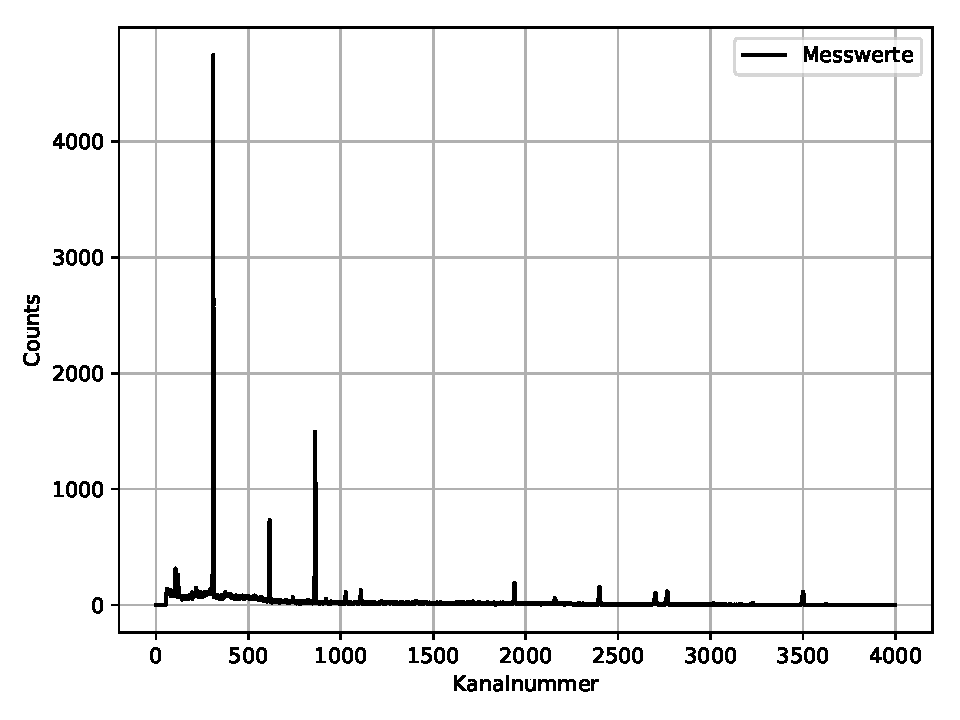
\includegraphics[height=9cm]{Eu.pdf}
  \caption{Spektrum des $\ce{^{152}Eu}$-Strahlers}
  \label{fig:plot1}
\end{figure}

Um mit diesem die Energiekalibration durchzuführen, werden die Peaks des Spektrums
jeweils mit einer Gaußverteilung der Form
\begin{equation}
  \symup{g} (x) = a + b \cdot \symup{e}^{(\frac{x-z}{c})^2}
  \label{eqn:gausk}
\end{equation}
gefittet.

Die sich daraus ergebenen Parameter sind in Tabelle \ref{tab:tabe1} angegebenen.
\begin{table}[H]
  \centering
  \caption{Messwerte der Wärmepumpe}
  \label{tab:tabe1}
    \begin{tabular}{S S S S S S}
    \toprule
    $ t  \: / \si{\second} $ & $ p_a \: / \si{\bar} $ & $ p_b \: / \si{\bar} $ &
    $ T_1 \: / \si{\kelvin} $ & $ T_2 \: / \si{\kelvin} $ & $ P \: / \: \si{\watt} $\\
    \midrule
    0 & 5.0 & 5.0 & 293.65 & 293.65 & 0 \\
    60 & 4.7 & 6.0 & 294.15 & 293.55 & 115 \\
    120 & 4.4 & 6.4 & 295.15 & 293.15 & 118 \\
    180 & 4.5 & 6.9 & 296.35 & 291.95 & 122 \\
    240 & 4.6 & 7.0 & 297.55 & 290.95 & 125 \\
    300 & 4.6 & 7.0 & 298.85 & 289.95 & 125 \\
    360 & 4.5 & 7.2 & 300.05 & 289.15 & 123 \\
    420 & 4.4 & 7.4 & 301.15 & 288.45 & 123 \\
    480 & 4.3 & 7.8 & 302.35 & 287.65 & 122 \\
    540 & 4.2 & 8.0 & 303.55 & 286.95 & 122 \\
    600 & 4.2 & 8.1 & 304.65 & 286.25 & 121 \\
    660 & 4.1 & 8.3 & 305.75 & 285.55 & 121 \\
    720 & 4.0 & 8.5 & 306.75 & 284.95 & 121 \\
    780 & 4.0 & 8.8 & 307.75 & 284.35 & 121 \\
    840 & 3.9 & 9.0 & 308.75 & 283.75 & 121 \\
    900 & 3.8 & 9.1 & 309.65 & 283.15 & 121 \\
    960 & 3.8 & 9.2 & 310.55 & 282.55 & 122 \\
    1020 & 3.8 & 9.5 & 311.45 & 282.05 & 122 \\
    1080 & 3.7 & 9.8 & 312.25 & 281.55 & 122 \\
    1140 & 3.7 & 10.0 & 313.05 & 281.15 & 122 \\
    1200 & 3.7 & 10.0 & 313.9 & 280.65 & 122 \\
    1260 & 3.6 & 10.2 & 314.65 & 280.25 & 123 \\
    1320 & 3.6 & 10.3 & 315.35 & 279.85 & 123 \\
    1380 & 3.6 & 10.6 & 316.15 & 279.45 & 124 \\
    1440 & 3.6 & 10.8 & 316.85 & 279.15 & 124 \\
    1500 & 3.6 & 11.0 & 317.55 & 278.75 & 124 \\
    1560 & 3.6 & 11.1 & 318.25 & 278.55 & 124 \\
    1620 & 3.6 & 11.2 & 318.95 & 278.25 & 125 \\
    1680 & 3.5 & 11.4 & 319.55 & 277.95 & 125 \\
    1740 & 3.5 & 11.5 & 320.15 & 277.65 & 125 \\
    1800 & 3.5 & 11.7 & 320.75 & 277.45 & 125 \\
    1860 & 3.5 & 11.9 & 321.35 & 277.25 & 125 \\
    1920 & 3.5 & 12.0 & 321.95 & 277.05 & 125 \\
    1980 & 3.5 & 12.1 & 322.45 & 276.95 & 125 \\








      \bottomrule
    \end{tabular}
\end{table}


Die zentrale Lage der Peaks im Hinblick auf die Kanalnummer ist durch den Parameter
z gegeben. Diese werden zusammen mit der jeweiligen relativen Höhe mit den theoretischen
Emissionslinien der Datenbank \cite{lara} verglichen und es wird jedem Peak eine Linie
zugeordent. Diese Zuordnung ist zusammen mit der jeweiligen relativen Emissionswahrscheinlichkeit P
in Tabelle \ref{tab:tabe2} dargestellt.
\begin{table}[H]
  \centering
  \caption{Wertetabelle für $\alpha$ und $C_V$.}
  \label{tab:tab2}
    \begin{tabular}{S S S S S}
    \toprule
    $ T\: \text{in}\: \si{\K} $ & $ {\alpha \cdot 10^{-6} \: \text{in}\: \si {\per\K}} $ &
    $ C_V \: \text{in}\: \si{\J\per\K\mol} $\\
    \midrule %Cv, a *10-6, Cv
    %0 & 1 & 1\\
    88.60\pm0.24 & 9.56\pm0.06 & 14.17\pm8.13  \\ %&3.6 & 318.97\pm0.85\\
    93.81\pm0.24 & 10.10\pm0.06 & 17.58\pm10.03 \\ %& 4.7 & 440.90\pm1.11\\
    99.74\pm0.24 & 10.66\pm0.05 & 15.52\pm8.84 \\ %& 5.1 & 508.68\pm1.21\\
    104.74\pm0.24 & 11.07\pm0.05 & 18.44\pm10.52 \\ %& 4.6 & 481.79\pm1.09\\
    110.94\pm0.24 &  11.54\pm0.05 & 14.86\pm8.45 \\ %& 5.3 & 587.97\pm1.27\\
    115.96\pm0.24 & 11.89\pm0.05 & 18.49\pm10.52 \\ %& 4.6 & 533.41\pm1.10\\
    121.47\pm0.24 &  12.22\pm0.05 & 16.83\pm9.57 \\ %& 4.9 & 595.21\pm1.17\\
    126.99\pm0.24 & 12.53\pm0.04 & 16.79\pm9.54 \\ %& 4.9 & 622.29\pm1.18\\
    131.58\pm0.24 & 12.77\pm0.04 & 20.42\pm11.62 \\ %& 4.2 & 552.62\pm1.01\\
    136.65\pm0.24 & 13.02\pm0.04 & 18.40\pm10.47 \\ %& 4.6 & 628.57\pm1.11\\
    141.49\pm0.24 & 13.24\pm0.04 & 19.28\pm10.97 \\ %& 4.4 & 622.54\pm1.07\\
    146.34\pm0.24 & 13.44\pm0.04 & 19.24\pm10.95 \\ %& 4.4 & 643.88\pm1.07\\
    150.95\pm0.24 & 13.62\pm0.04 & 20.22\pm11.52 \\ %& 4.3 & 649.11\pm1.05\\
    155.34\pm0.24 & 13.79\pm0.04 & 21.31\pm12.14 \\ %& 4.1 & 636.88\pm0.98\\
    159.97\pm0.24 & 13.95\pm0.04 & 20.12\pm11.47 \\ %& 4.3 & 687.89\pm1.05\\
    164.62\pm0.24 & 14.10\pm0.04 & 20.18\pm11.51 \\ %& 4.3 & 707.87\pm1.06\\
    168.79\pm0.25 & 14.23\pm0.04 & 22.54\pm12.86 \\ %& 3.9 & 658.27\pm0.95\\
    173.45\pm0.25 &  14.37\pm0.04 & 20.08\pm11.46 \\ %& 4.3 & 745.84\pm1.06\\
    178.13\pm0.25 &  14.50\pm0.04 & 20.04\pm11.44 \\ %& 4.3 & 765.94\pm1.06\\
    182.56\pm0.25 &  14.62\pm0.04 & 21.11\pm12.06\\
    192.70\pm0.25 &  14.87\pm0.04 & 18.41\pm10.47\\
    200.15\pm0.25 &  15.04\pm0.04 & 25.19\pm14.28\\
    208.87\pm0.25 &  15.23\pm0.04 & 21.43\pm12.18\\
    217.12\pm0.25 &  15.38\pm0.04 & 22.65\pm12.88\\
    225.15\pm0.25 &  15.53\pm0.03 & 23.27\pm13.24\\
    232.70\pm0.25 &  15.70\pm0.03 & 24.75\pm14.08\\
    240.53\pm0.25 &  15.74\pm0.03 & 23.84\pm13.58\\
    248.39\pm0.25 &  15.89\pm0.03 & 23.74\pm13.53& \\
    256.01\pm0.25 &  15.97\pm0.03 & 24.46\pm13.94 \\
    263.41\pm0.26 &  16.01\pm0.03 & 25.22\pm14.38 \\
    271.08\pm0.26 &  16.18\pm0.03 & 24.26\pm13.86 \\
    278.52\pm0.26 &  16.27\pm0.03 & 25.03\pm14.29&\\
    285.98\pm0.26 &  16.35\pm0.03 & 24.92\pm14.25 \\
    293.21\pm0.26 &  16.42\pm0.03 & 25.74\pm14.72 \\
    300.98\pm0.26 &  16.50\pm0.03 & 23.87\pm13.68 \\
    308.51\pm0.26 &  16.57\pm0.03 & 24.63\pm14.12\\



      \bottomrule
    \end{tabular}
\end{table}

Mit den Wertepaaren aus Kanalnummer und Linienenergie wird nun eine lineare Ausgleichsrechnung der
Form
\begin{equation*}
  f(x) = a\cdot x +b
\end{equation*}
durchgeführt, woraus sich die Parameter
\begin{align}
  a = \SI{0.403169(29)}{\kilo\electronvolt} \\
  b = \SI{-3.034(60)}{\kilo\electronvolt}
\end{align}
ergeben. Die Wertepaare sind zusammen mit der resultierenden Gerade in Abbildung \ref{fig:plot3}
dargestellt. Die Fehler der Messwerte sind aufgrund ihrer sehr geringen relativen Größe dabei zu vernachlässigen.
\begin{figure}
  \centering
  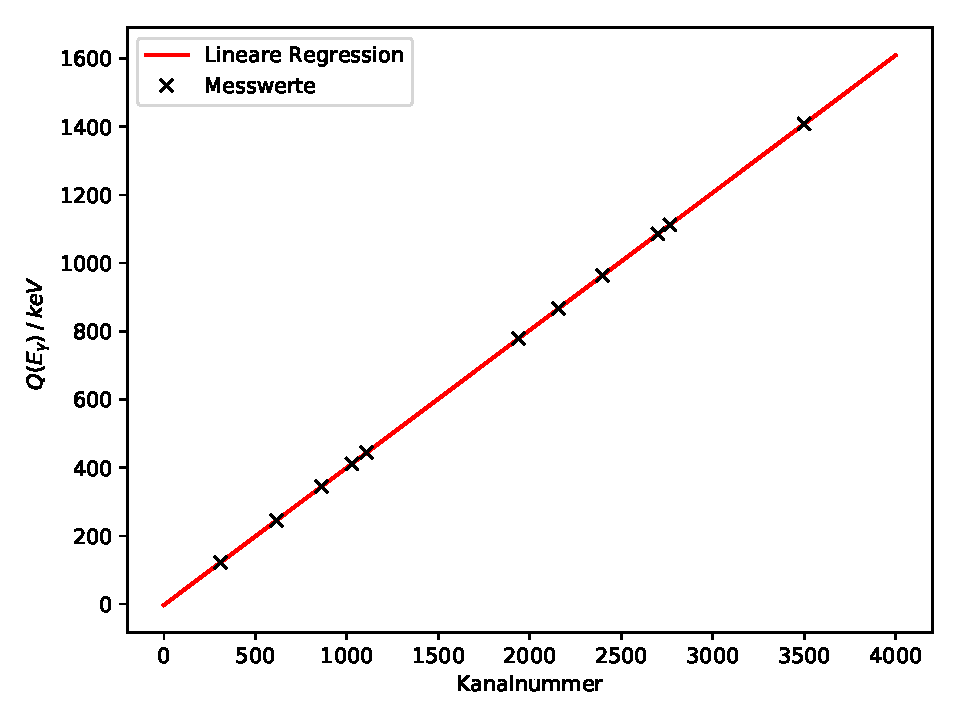
\includegraphics[height=9cm]{plot3.pdf}
  \caption{Lineare Ausgleichsrechnung zur Energiekalibration}
  \label{fig:plot3}
\end{figure}
Die Energiekalibration erfolgt somit gemäß
\begin{equation}
  \symup{E}_{\gamma} (x) = \SI{0.403169}{\kilo\electronvolt}\cdot x
  \label{eqn:gerade}
\end{equation}
wobei x die Kanalnummer bezeichnet.
Der dazugehörige Fehler ergibt mittels Gleichung \ref{eqn:gaus} durch
\begin{equation}
   \increment \symup{E}_{\gamma} (x) =\sqrt{ (\SI{0.000029}{\kilo\electronvolt}\cdot x)^2 +
   (\SI{60}{\kilo\electronvolt})^2}
   \label{eqn:fgerade}
\end{equation}
\\
Zur Bestimmung der Vollenergienachweiswahrscheinlichkeit wird zunächst die Gleichung \ref{eqn:gausk}
integriert, um den Inhalt der Peaks zu bestimmen, wobei der Untegrund $a$ vorher abgezogen wird.
Es ergibt sich somit ein Linieninhalt von
\begin{equation}
  \symup{I} =\int_{-\infty}^{\infty} c \cdot \symup{e}^{(\frac{x-z}{b})^2} \symup{d}x
  = c \cdot b \cdot \sqrt{\pi}
  \label{eqn:inh}
\end{equation}
in Abhängigkeit der Parameter b und c.
Der Fehler ergibt sich durch Gleichung \ref{eqn:gaus} über die Gleichung
\begin{equation}
  \increment \symup{I} = \sqrt{ (\increment c \cdot b \cdot \sqrt{\pi})^{2}
   + (c \cdot \increment b \cdot \sqrt{\pi}})^{2} \: .
     \label{eqn:inhf}
\end{equation}
Mit den Werten aus Tabelle \ref{tab:tabe1} lassen sich somit die einzelnen Linieninhalte berrechen,
welche in Tabelle \ref{tab:tabe3} angegeben sind.
\begin{table}
  \centering
  \caption{Messwerte für den ersten Doppelspalt.}
   \begin{tabular}{S S| S S | S S}
    \toprule
    $x/\; \si{\mm}$& $A/\;\si{\nA}$ &
    $x/\; \si{\mm}$& $A/\;\si{\nA}$ &
    $x/\; \si{\mm}$& $A/\;\si{\nA}$ \\
    \midrule

    15.0& 4.6& 23.0& 25.0& 29.5& 6.0\\
    15.5& 4.2& 23.5& 30.0& 30.0& 5.3\\
    16.0& 4.0& 24.0& 35.0& 30.5& 4.9\\
    16.5& 4.0& 24.25& 36.0& 31.0& 4.7\\
    17.0& 4.4& 24.5& 37.0& 31.5& 4.4\\
    17.5& 5.5& 24.75& 38.0& 32.0& 4.2\\
    18.0& 6.6& 25.00& 37.0& 32.5& 3.8\\
    18.5& 7.7& 25.25& 36.0& 33.0& 3.6\\
    19.0& 8.2& 25.5& 36.0& 33.5& 3.2\\
    19.5& 8.4& 26.0& 33.0& 34.0& 3.2\\
    20.0& 8.4& 26.5& 28.5& 34.5& 3.2\\
    20.25& 8.4& 27.0& 23.0& 35.0& 3.3\\
    20.5& 8,7& 27.5& 18.0& 35.5& 3.4\\
    21.0& 9.8& 28.0& 13.5& 36.0& 3.5\\
    21.5& 12.0& 28.5& 10.0\\
    22.0& 15.0& 29.0& 7.8\\
    22.5& 20.0& 29.25& 6.7\\


   \bottomrule
  \end{tabular}
  \label{tab:tabelle3}
\end{table}

Zum Vergleich werden nun die Theoriewerte berrechnet, als Produkt
der Emissionswahrscheinlichkeiten P aus Tabelle \ref{tab:tabe2},
dem abgedeckten Raumwinkelanteil $\frac{\Omega}{4\pi}= 0.01558$, der errechneten Aktivität
$A =\SI{1599(29)}{\becquerel} $
und der Messzeit von $t = \SI{3598}{\second}$
\begin{equation}
  \symup{I}_{\text{theo}} = P\cdot \frac{\Omega}{4\pi} \cdot A \cdot t
\end{equation}
mit dem Fehler über Gleichung \ref{eqn:gaus} von
\begin{equation}
  \increment \symup{I}_{\text{theo}} = \sqrt{ (\increment P\cdot \frac{\Omega}{4\pi} \cdot A \cdot t)^{2}
   + (P\cdot \frac{\Omega}{4\pi} \cdot \increment A \cdot t)^{2}} \: .
\end{equation}
Aus dem jeweiligen Quotienten
\begin{equation}
  \symup{Q} = \frac{\symup{I}}{\symup{I}_{\text{theo}}}
\end{equation}
mit dem dazugehörigen Fehler
\begin{equation}
  \increment \symup{Q} = \sqrt{ (\frac{1}{\symup{I}_{\text{theo}} \cdot \increment \symup{I})^{2}
   + (\frac{\symup{I}}{\symup{I}_{\text{theo}}})^{2}}\cdot \increment \symup{I}_{\text{theo}})^{2}}
\end{equation}
ergibt sich somit jeweils die Nachweiswahrscheinlichkeit des Peaks, wie in Tabelle
\ref{tab:tabe4} dargestellt ist.
\begin{table}[H]
  \centering
   \begin{tabular}{c c c c}
    \toprule
    Nummer der Oberwelle & $ U_{\text Theorie,Rechteck}\: / \si{\volt} $ &
    $ U_{\text Theorie,Dreick}\: / \si{\volt} $ & $ U_{\text Theorie,Sägezahn}\: / \si{\volt} $ \\
    \midrule
    1 & 1145 & 182 & 573 \\
    2 & 0 & 0 & 286 \\
    3 & 573 & 20 & 191 \\
    4 & 0 & 0 & 143 \\
    5 & 229 & 7 & 115 \\
    6 & 0 & 0 & 96 \\
    7 & 164 & 4 & 82 \\
    8 & 0 & 0 & 72 \\
    9 & 127 & 2 & 64 \\
    10 & 0 & 0 & 57 \\
    \bottomrule
  \end{tabular}
  \caption{Eingestellte Schwingungsamplituden.}
  \label{tab:tabe4}
\end{table}

Da die Nachweiswahrscheinlichkeit im Allgemeinen energieabhängig ist, wird Q in
Abhängigkeit von $ \text{E}_{\gamma} $ dargestellt und mit einer Potenzfunktion der Form
\begin{equation}
  \symup{Q}(\text{E}_{\gamma}) = c\cdot (\text{E}_{\gamma}-a)^{d}
\end{equation}
gefittet, wie in Abbildung \ref{fig:plot4} dargestellt ist.
Es ergeben sich hierbei die Parameter

\begin{align*}
  a = -191 \pm 64\\
  c = 2474 \pm 3467\\
  d = -1.47 \pm 0.19\:,
\end{align*}

welche zum Teil mit einem großen Fehler behaftet sind.
\begin{figure}
  \centering
  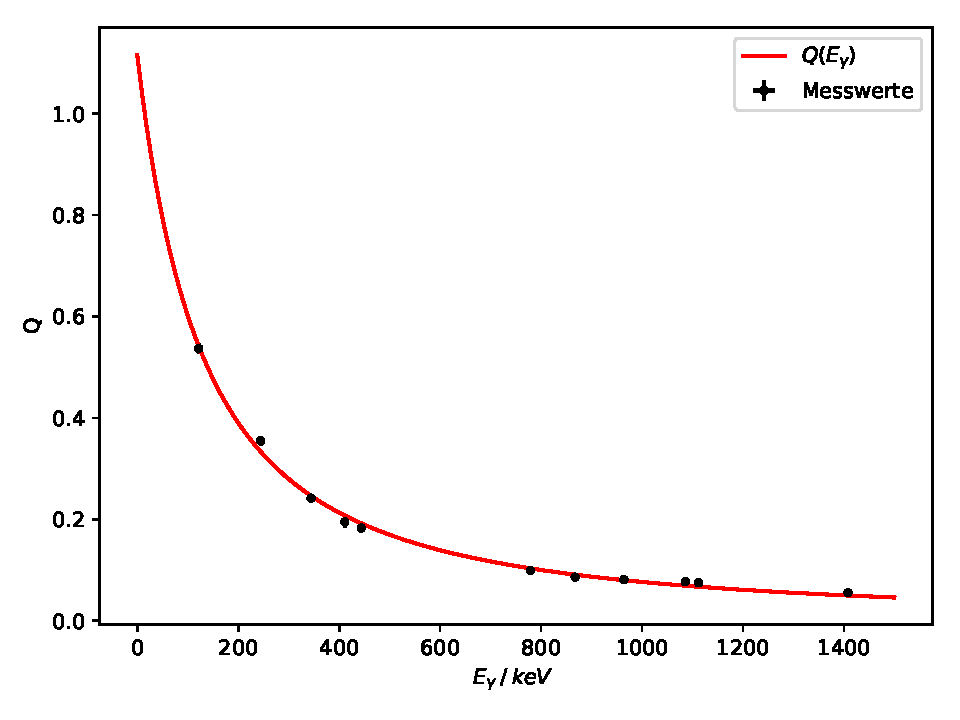
\includegraphics[height=9cm]{plot4.pdf}
  \caption{Werte zur Bestimmung der Vollenergienachweiswahrscheinlichkeit sowie gefittete Potenzfunktion}
  \label{fig:plot4}
\end{figure}

\section{Untersuchung eines monochromatischen Gamma-Spektrums}
Zur Untersuchung des monochromatischen Gamma-Spektrums wird das aufgenommene Spektrum
zunächst durch die Gleichung \ref{eqn:gerade} kalibriert, wobei sich der Fehler über
\ref{eqn:fgerade} ergibt. Die so erhaltenen Werte sind in Abbildung \ref{fig:plot5}
dargestellt, wobei auf Fehlerbalken aufgrund der geringen Fehler verzichtet wurde. Die
Messzeit beträgt $\SI{2593}{\second}$ und es wurden 8191 Kanäle gemessen, wobei nur die
ersten 2000 dargestellt sind, da bei höheren Kanalnummern keine signifikanten Messwerte
mehr zu erkennen sind.
\begin{figure}
  \centering
  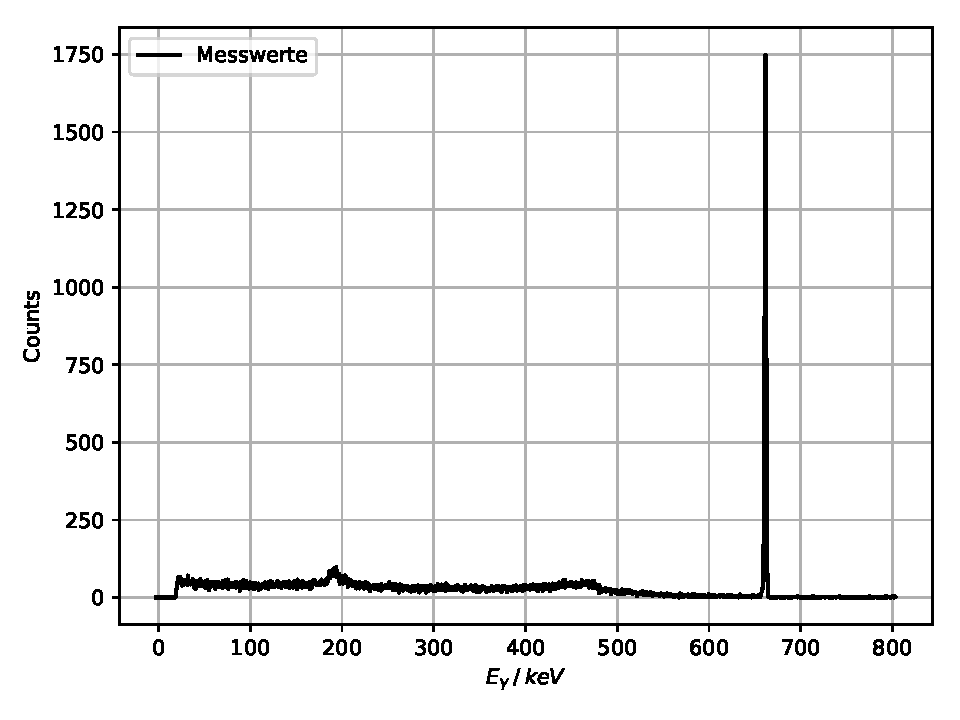
\includegraphics[height=9cm]{Cs.pdf}
  \caption{Kalibriertes Spektrum des $\ce{^{137}Cs}$-Strahlers }
  \label{fig:plot5}
\end{figure}
Zur Bestimmung der Energie wird die Vollenergielinie mit der Gaußverteilung aus Gleichung
\ref{eqn:gausk} gefittet, wobei sich die Parameter
\begin{align*}
  a = 5.7 \pm 4.2 \\
  b = 1674 \pm 17 \\
  c = \SI{1.227(15)}{\kilo\electronvolt}\\
  z = \SI{661.5985(98)}{\kilo\electronvolt} \:
\end{align*}
ergeben.
Die Energie des Strahlers ist dabei durch den Parameter $z$ gegeben, also
\begin{align*}
  \symup{E}_{Cs} = \SI{661.5985(98)}{\kilo\electronvolt} \: .
\end{align*}
Der Bereich um die Vollenergielinie ist zusammen mit der gefitteten Gaußkurve in
Abbildung \ref{fig:plot6} dargestellt.
\begin{figure}
  \centering
  \includegraphics[height=9cm]{Plot6.pdf}
  \caption{Vollenergielinie mit Gaußkurve}
  \label{fig:plot6}
\end{figure}
Die Halbwertsbreite einer Gaußkurve gemäß Gleichung \ref{eqn:gausk} ist durch die
Formel
\begin{equation}
  \symup{E}_{1/2} = 2c*\sqrt{ln2}
\end{equation}
mit dem Fehler
\begin{equation}
  \increment \symup{E}_{1/2} = 2\increment b*\sqrt{ln2} \: ,
\end{equation}
gegeben und beträgt somit
\begin{align*}
  \symup{E}_{1/2} = \SI{1.701(21)}{\kilo\electronvolt} \: .
\end{align*}
Die Zehntelwertsbreite ergibt sich analog über die Gleichung
\begin{equation}
  \symup{E}_{1/10} = 2c*\sqrt{ln10}
\end{equation}
mit dem Fehler
\begin{equation}
  \increment \symup{E}_{1/10} = 2\increment b*\sqrt{ln10} \: ,
\end{equation}
zu
\begin{align*}
  \symup{E}_{1/10} = \SI{5.651(69)}{\kilo\electronvolt} \: .
\end{align*}
Der Inhalt der Vollenergielinie ergibt sich erneut durch Gleichungen \ref{eqn:inh}
und \ref{eqn:inhf} zu
\begin{align*}
  \symup{I}_{VEL} =  3641 \pm 58 \: .
\end{align*}
\\
Aus den Messwerten und Abbildung \ref{fig:plot5} lässt sich erkennen, dass die
Compton-Kante bei etwa $\SI{478}{\kilo\electronvolt}$ liegt, da dort das Spektrum ein lokales
Maximum animmt und anschließend abfällt.
Der Rückstreupeak wird erneut mit der Gleichung \ref{eqn:gausk} gefittet, wodurch sich
die Parameter
\begin{align*}
  a = 65.8 \pm 2.0 \\
  b = 36 \pm 28 \\
  c = \SI{0.28(28)}{\kilo\electronvolt}\\
  z = \SI{193.78(24)}{\kilo\electronvolt} \:
\end{align*}
ergeben, der Rückstreupeak liegt also bei $\SI{193.78(24)}{\kilo\electronvolt}$.
